\documentclass[tikz,border=5pt]{standalone}
\usepackage[utf8]{vietnam}
\usepackage{amsmath,amssymb}
\usepackage{tikz}
\usetikzlibrary{shapes.geometric}

\begin{document}
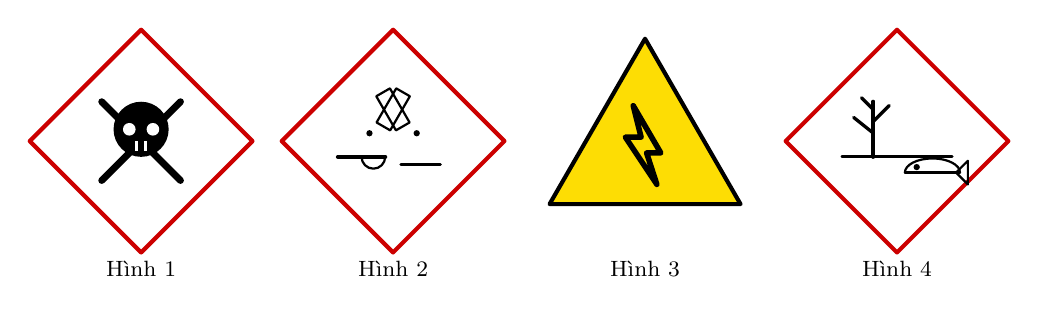
\begin{tikzpicture}[font=\footnotesize, line join=round, line cap=round]
    % Hình 1: Độc cấp tính (Đầu lâu xương chéo)
    \begin{scope}[shift={(0,0)}]
        \draw[line width=1.5pt, red!80!black, fill=white, rotate=45] (-1,-1) rectangle (1,1);
        % Xương chéo
        \draw[line width=2.5pt, black] (-0.5,-0.5) -- (0.5,0.5);
        \draw[line width=2.5pt, black] (-0.5,0.5) -- (0.5,-0.5);
        % Đầu lâu
        \fill[black] (0,0.15) circle (0.35);
        \fill[black] (-0.18,-0.15) rectangle (0.18,0.1);
        \fill[white] (-0.15,0.15) circle (0.08);
        \fill[white] (0.15,0.15) circle (0.08);
        \fill[white] (-0.08,-0.12) rectangle (-0.04,0);
        \fill[white] (0.04,-0.12) rectangle (0.08,0);
        \node[below] at (0,-1.4) {Hình 1};
    \end{scope}

    % Hình 2: Ăn mòn
    \begin{scope}[shift={(3.2,0)}]
        \draw[line width=1.5pt, red!80!black, fill=white, rotate=45] (-1,-1) rectangle (1,1);
        % Ống nghiệm đổ hóa chất
        \draw[thick, rotate=-30] (-0.3,0.6) rectangle (-0.1,0.1);
        \draw[thick, rotate=30] (0.1,0.6) rectangle (0.3,0.1);
        % Giọt hóa chất
        \fill[black] (-0.3,0.1) circle (0.04);
        \fill[black] (0.3,0.1) circle (0.04);
        % Bề mặt bị ăn mòn & bàn tay
        \draw[line width=1.5pt] (-0.7,-0.2) -- (-0.1,-0.2);
        \draw[line width=1.2pt] (0.1,-0.3) -- (0.6,-0.3);
        \draw[thick] (-0.4,-0.2) arc (180:360:0.15);
        \node[below] at (0,-1.4) {Hình 2};
    \end{scope}

    % Hình 3: Nguy cơ điện giật (Tam giác vàng)
    \begin{scope}[shift={(6.4,0)}]
        \node[regular polygon, regular polygon sides=3, draw=black, line width=1.5pt, fill=yellow!80!orange, minimum size=2.8cm, inner sep=0] at (0,-0.1) {};
        % Tia sét
        \draw[line width=2pt, black] (-0.15,0.45) -- (-0.05,0.05) -- (-0.25,0.05) -- (0.15,-0.55) -- (0.02,-0.15) -- (0.2,-0.15) -- cycle;
        \node[below] at (0,-1.4) {Hình 3};
    \end{scope}

    % Hình 4: Nguy hại môi trường (Cây khô và cá chết)
    \begin{scope}[shift={(9.6,0)}]
        \draw[line width=1.5pt, red!80!black, fill=white, rotate=45] (-1,-1) rectangle (1,1);
        % Mặt nước / mặt đất
        \draw[line width=1pt] (-0.7,-0.2) -- (0.7,-0.2);
        % Cây khô
        \draw[line width=1.5pt] (-0.3,-0.2) -- (-0.3,0.5);
        \draw[line width=1.2pt] (-0.3,0.1) -- (-0.55,0.3);
        \draw[line width=1.2pt] (-0.3,0.25) -- (-0.1,0.45);
        \draw[line width=1.2pt] (-0.3,0.4) -- (-0.45,0.55);
        % Con cá chết nằm ngửa
        \draw[thick] (0.1,-0.4) arc (180:0:0.35 and 0.18);
        \draw[thick] (0.1,-0.4) -- (0.8,-0.4);
        \draw[thick] (0.75,-0.4) -- (0.9,-0.25) -- (0.9,-0.55) -- cycle;
        \fill (0.25,-0.33) circle (0.04);
        \node[below] at (0,-1.4) {Hình 4};
    \end{scope}
\end{tikzpicture}
\end{document}
